\pdfminorversion=4
\documentclass[aspectratio=169]{beamer}
\usepackage{animate} % for animation
\usepackage{array,multirow,graphicx}
\usepackage{multicol}
\usepackage{etoolbox}
\graphicspath{{gambar/}}
\setbeamertemplate{caption}[numbered]
\setbeamertemplate{section in toc}[sections numbered]

% Hide subsubsections from TOC, but keep PDF bookmarks with beamer
\hypersetup{bookmarksopen=true,bookmarksopenlevel=4}
\setcounter{tocdepth}{4}

\renewcommand{\figurename}{Gambar.}
\renewcommand{\tablename}{Tabel.}

\usetheme[pageofpages=of,	% String used between the current page and the
							% total page count.
			alternativetitlepage=true,% Use the fancy title page.
			titleline=true,
			titlepagelogo=OK-LOGO-ITK.jpg
%          	 titlepagelogo=fig/jaist_logo.png
			]{Torino}
			% change /beamerinnerthemefancy.sty to resize the logo
\usecolortheme{freewilly}

\makeatletter
\patchcmd{\beamer@sectionintoc}{\vskip1.5em}{\vskip0em}{}{}
\makeatother

\author{Mifta Nur Farid, S.T., M.T. \\
	miftanurfarid@lecturer.itk.ac.id}
\title{RANGKAIAN ELEKTRONIKA II}
\subtitle{Negative Feedback}
\institute{Teknik Elektro \\ Institut Teknologi Kalimantan \\ Balikpapan, Indonesia}
\date{\tiny Maret 10, 2021}

% The log drawn in the upper right corner.
\logo{
\includegraphics[height=0.13\paperheight]{OK-LOGO-ITK.jpg}}

\begin{document}

\begin{frame}[t,plain]
\titlepage
\end{frame}

\section{Sub-CPMK}
\begin{frame}{Sub-CPMK}
	Mahasiswa mampu memperbandingkan keempat jenis negative feedback (C5, P4, A4)
\end{frame}

\section{Bahan Kajian}
\begin{frame}{Bahan Kajian}
	\begin{enumerate}
		\item Konsep dasar negative feedback;
		\item VCVS voltage gain;
		\item ICVS amplifier;
		\item VCIS amplifier;
		\item ICIS amplifier.
	\end{enumerate}
\end{frame}
\section{Pengantar Negative Feedback}

\subsection{Empat Jenis Negative Feedback}	
\begin{frame}{Empat Jenis Negative Feedback}	
	\begin{itemize}
		\item Negative feeback pertama $ \rightarrow $ menstabilkan voltage gain, meningkatkan impedansi input, menurunkan impedansi output
		\item Dengan adanya transistor \& op amps $\rightarrow$ bertambah 3 jenis negative feedback
	\end{itemize}
\end{frame}

\subsection{Ide Dasar}
\begin{frame}{Ide Dasar}
	\begin{itemize}
		\item Input dan output negative feedback amplifier bisa berupa tegangan maupun arus $ \rightarrow $ 4 tipe negative feedback
	\end{itemize}
	\begin{center}
		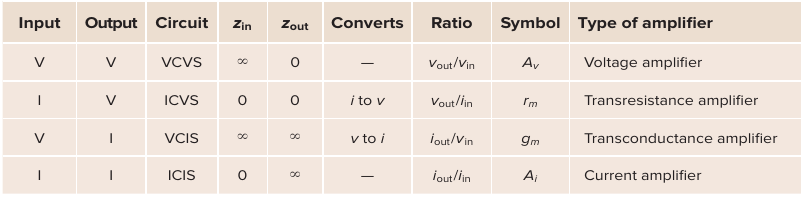
\includegraphics[width=\linewidth]{gambar/table-17.01}
	\end{center}
\end{frame}

\begin{frame}{Ide Dasar}
	\begin{itemize}
		\item \textbf{Jenis 1}: tegangan input dan tegangan output
		\begin{itemize}
			\item Rangkaian yang menggunakan negative feedback jenis ini disebut \textbf{voltage-controlled voltage source (VCVS)}
			\item Merupakan ideal voltage amplifier $ \rightarrow $ menstabilkan voltage gain, impedansi input tak hingga, impedansi output nol
		\end{itemize}
	
		\item \textbf{Jenis 2}: Arus input mengendalikan tegangan output
		\begin{itemize}
			\item Rangkaian yang menggunakan negative feedback jenis ini disebut \textbf{current-controlled voltage source (ICVS)}
			\item Disebut juga \textbf{transresistance amplifier} karena rasio dari $ v_{out}/i_{in} $ memliki satuan ohm
		\end{itemize}
	\end{itemize}
\end{frame}

\begin{frame}{Ide Dasar}
	\begin{itemize}	
		\item \textbf{Jenis 3}: Tegangan input mengendalikan arus output
		\begin{itemize}
			\item Rangkaian yang menggunakan negative feedback jenis ini disebut \textbf{voltage-controlled current source (VCIS)}
			\item Disebut juga \textbf{transconductance amplifier} karena rasio dari $ i_{out}/v_{in} $ memliki satuan mho
		\end{itemize}
		
		\item \textbf{Jenis 4:} Arus input dikuatkan untuk mendapatkan arus output yang lebih besar
		\begin{itemize}
			\item Rangkaian yang menggunakan negative feedback jenis ini disebut \textbf{current-controlled current source (ICIS)}
			\item Merupakan ideal current amplifier karena menstabilkan current gain, impedansi input nol dan impedansi ouput tak hingga
		\end{itemize}
	\end{itemize}
\end{frame}

\subsection{Konverter}
\begin{frame}{Konverter}
	\begin{itemize}
		\item Rangkaian VCVS dan ICIS disebut sebagai amplifier $ \rightarrow $ make sense, karena VCVS = voltage amplifier dan ICIS = current amplifier
		\item Namun bagaimana dengan transconductance dan transresistance amplifier ? $ \rightarrow $ input dan outputnya berbeda
		\item Rangkaian transconductance dan transresistance amplifier $ \rightarrow $ converter
		\item VCIS $\rightarrow$ voltage-to-current converter
		\item ICVS $\rightarrow$ current-to-voltage converter
	\end{itemize}
\end{frame}

\subsection{Diagram}
\begin{frame}{Diagram}
	\begin{figure}
		\centering
		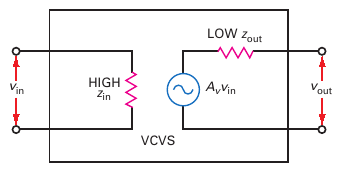
\includegraphics[width=0.7\linewidth]{gambar/fig-17.01a}
		\caption{Voltage-controlled voltage source}
		\label{fig-17.01a}
	\end{figure}
\end{frame}

\begin{frame}{Diagram}
	\begin{figure}
		\centering
		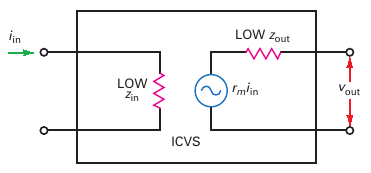
\includegraphics[width=0.7\linewidth]{gambar/fig-17.01b}
		\caption{Current-controlled voltage source}
		\label{fig-17.01b}
	\end{figure}
\end{frame}

\begin{frame}{Diagram}
	\begin{figure}
		\centering
		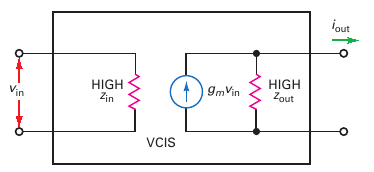
\includegraphics[width=0.7\linewidth]{gambar/fig-17.02a}
		\caption{Voltage-controlled current source}
		\label{fig-17.02a}
	\end{figure}
\end{frame}

\begin{frame}{Diagram}
	\begin{figure}
		\centering
		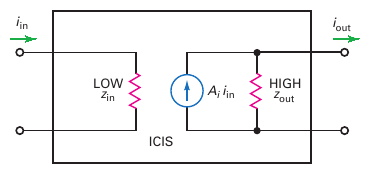
\includegraphics[width=0.7\linewidth]{gambar/fig-17.02b}
		\caption{Current-controlled current source}
		\label{fig-17.02b}
	\end{figure}
\end{frame}
\section{VCVS Voltage Gain}

\subsection{VCVS Voltage Gain}
\begin{frame}{Pengantar VCVS Voltage Gain}
	\begin{itemize}
		\item Sebelumnya kita telah menganalisa noninverting amplifier, sebuah implementasi secara luas dari VCVS.
		\item Pada bab ini, kita akan memeriksa kembali noninverting amplifier dan menggali lebih dalam terkait voltage gain-nya.
	\end{itemize}
\end{frame}

\subsection{Exact Closed-Loop Voltage Gain}
\begin{frame}{Exact Closed-Loop Voltage Gain}
	\begin{figure}
		\centering
		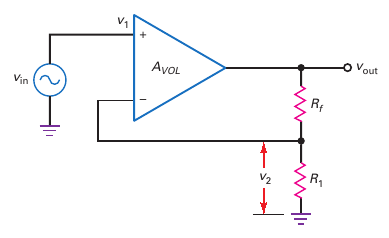
\includegraphics[height=0.7\textheight]{gambar/fig-17.03}
		\caption{VCVS amplifier / noninverting amplifier}
		\label{fig-17.03}
	\end{figure}
\end{frame}


\begin{frame}{Exact Closed-Loop Voltage Gain}
	\begin{itemize}
		\item Sebuah op amp biasanya memiliki open-loop voltage gain ($ A_{VOL} $) sebesar 100000 bahkan lebih.
		\item Karena ada pembagi tegangan maka sebagian dari tegangan output diumpankan kembali ke inverting input.
		\item Feedback fraction atau feedback attenuation factor: mengindikasikan berapa banyak tegangan keluaran teratenuasi sebelum sinyal feedback mencapai inverting input.
		\item Persamaan feedback fraction adalah
		\begin{equation}\label{pers-17.01}
			B = \frac{v_2}{v_{out}}
		\end{equation}
	\end{itemize}
\end{frame}

\begin{frame}{Exact Closed-Loop Voltage Gain}
	\begin{itemize}
		\item Closed-loop voltage gain:
		\begin{equation}\label{pers-17.02}
			A_{v(CL)} = \frac{A_{VOL}}{1 + A_{VOL}B}
		\end{equation}
		\item Berdasarkan Gambar \ref{tabel-17.1}, $ A_v = A_{v(CL)} $, maka exact closed-loop voltage gain dari setiap VCVS:
		\begin{equation}\label{pers-17.03}
			A_v = \frac{A_{VOL}}{1 + A_{VOL}B}
		\end{equation}
	\end{itemize}
\end{frame}

\subsection{Loop Gain}
\begin{frame}{Loop Gain}
	\begin{itemize}
		\item Istilah dari $ A_{VOL} B$ adalah Loop Gain.
		\item Disebut loop gain karena voltage gain dari forward dan feedback path.
		\item Loop gain sangat penting dalam mendesain negative-feedback amplifier.
		\item Dalam praktiknya, loop gain dibuat sangat besar.
		\item Semakin besar loop gain maka semakin baik. Karena loop gain menstabilkan voltage gain dan memperbaiki gain stability, distortion, offset, impedansi input dan impedansi output
	\end{itemize}
\end{frame}

\subsection{Ideal Closed-Loop Voltage Gain}
\begin{frame}{Ideal Closed-Loop VOltage Gain}
	\begin{itemize}
		\item Agar VCVS bekerja dengan baik, maka loop gain harus jauh lebih besar daripada unity
	\end{itemize}

	\begin{equation}\label{pers-17.04}
		A_v = \frac{A_{VOL}}{1 + A_{VOL} B} \cong \frac{A_{VOL}}{A_{VOL} B} = \frac{1}{B}
	\end{equation}
	
	\begin{itemize}
		\item Exact closed-loop gain sedikit lebih kecil daripada ideal closed-loop gain.
		\item Jika perlu, kita dapat menghitung percent error antara nilai ideal dan exact:
	\end{itemize}

	\begin{equation}\label{pers-17.05}
		\% Error = \frac{100\%}{1 + A_{VOL} B}
	\end{equation}

	\begin{itemize}
		\item Misalkan: jika $ 1 + A_{VOL}B $ adalah 1000 atau 60 dB, maka error hanya 0.1 \%. Artinya nilai exact hanya 0.1 \% lebih kecil daripada nilai idealnya.
	\end{itemize}
\end{frame}

\subsection{Menggunakan Persamaan Ideal}
\begin{frame}{Menggunakan Persamaan Ideal}
	\begin{itemize}
		\item Persamaan \ref{pers-17.04} dapat digunakan untuk menghitung ideal closed-loop voltage gain dari setiap VCVS amplifier.
		\item Caranya dengan mengitung feedback fractiong menggunakan persamaan \ref{pers-17.03} kemudian ambil reciprocalnya
		\item Contohnya, berdasarkan Gambar \ref{fig-17.03}, feedback fraction:
		\begin{equation}\label{pers-17.06}
			V = \frac{v_2}{v_{out}} = \frac{R_1}{R_1 + R_f}
		\end{equation}\\
		Dengan mengambil reciprocalnya:
		\[ A_v \cong \frac{1}{B} = \frac{R_1 + R_f}{R_1} = \frac{R_f}{R_1} + 1 \]
	\end{itemize}
\end{frame}

\subsection{Contoh Soal 3.4}
\begin{frame}{Contoh Soal 3.4}
	\begin{multicols}{2}
		\begin{center}
			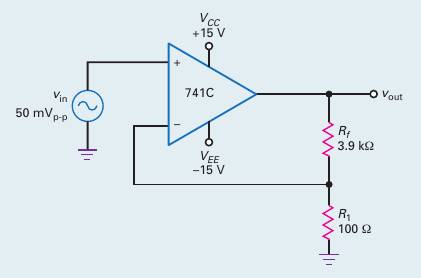
\includegraphics[width=1\linewidth]{gambar/fig-17.04}
		\end{center}
		\columnbreak
		\begin{itemize}
			\item Pertanyaan:
			\begin{itemize}
				\item Berdasarkan gambar di samping, jika $ A_{VOL} $ dari 741C adalah 100000, tentukan feedback fraction, ideal closed-loop voltage gain, percent error, dan exact closed-loop voltage gain.
			\end{itemize}
		\end{itemize}
	\end{multicols}
\end{frame}
\section{Current-Controlled Voltage Source (ICVS)}
\begin{frame}{Current-Controlled Voltage Source (ICVS)}
	content
\end{frame}
\section{Voltage-Controlled Current Source (VCIS)}
\begin{frame}{Voltage-Controlled Current Source (VCIS)}
	content
\end{frame}
\section{Current-Controlled Current Source (ICIS)}
\begin{frame}{Current-Controlled Current Source (ICIS)}
	content
\end{frame}
\begin{frame}
	\centering TERIMA KASIH
\end{frame}

\end{document}

